\documentclass[%
a4paper,
DIV12,
2.5headlines,
bigheadings,
titlepage,
openbib,
%draft
]{scrartcl}

%%% PACKAGES
\usepackage[ngerman, english]{babel}
%% FONTS


\usepackage[T1]{fontenc}
\usepackage{geometry}
\usepackage[latin1]{inputenc}
\usepackage{mathpazo}
\usepackage{helvet}
\usepackage{courier}
\usepackage{eurosym}
\usepackage{amsmath}
\usepackage{courier}
\usepackage{scrpage2}
\usepackage{graphicx}
\usepackage{xcolor}
\usepackage{multirow}
\usepackage{varioref}
\usepackage{babelbib}
\usepackage{makeidx}
\usepackage{tabularx}
\usepackage{floatflt}
\usepackage[pdftex, colorlinks, linktocpage, linkcolor=black, citecolor=black, urlcolor=black]{hyperref}

\graphicspath{ {images/} }

\pagestyle{scrheadings}


\geometry{a4paper, top=55mm, left=40mm, right=35mm, bottom=40mm,
headsep=10mm, footskip=22mm}
\linespread {1.25}
%%% COMMANDS

	%%%%%%%%%%%%%%%%%%
	% Autor eintragen
	\newcommand{\theauthor}{Markus Petrykowski}
	%%%%%%%%%%%%%%%%%%
	% Matrikelnummer eintragen
	\newcommand{\matrnr}{761918}
	%%%%%%%%%%%%%%%%%%
	% Titel eintragen
	\newcommand{\thetitle}{Identifying Future product needs by Clustering Companies}

%%% COLORS√
% Rot
\definecolor{hpired}{rgb}{0.686,0,0.204}
% Orange
\definecolor{hpiorange}{rgb}{0.867,0.380,0.031}	
% Gelb
\definecolor{hpiyellow}{rgb}{0.965,0.659,0}			%100 
\colorlet{hpiyellow2}{hpiyellow!60!white}				% 60
\colorlet{hpiyellow3}{hpiyellow!40!white}				% 40
\colorlet{hpiyellow4}{hpiyellow!20!white}				% 20
% Grau
\definecolor{hpigrey}{rgb}{0.376,0.408,0.420}		%100
\colorlet{hpigrey2}{hpigrey!70!white}						% 70
\colorlet{hpigrey3}{hpigrey!50!white}						% 50
\colorlet{hpigrey4}{hpigrey!20!white}						% 20
% Blau
\definecolor{hpiblue}{rgb}{0,0.478,0.620}				%100
\colorlet{hpiblue2}{hpiblue!60!white}						% 60
\colorlet{hpiblue3}{hpiblue!40!white}						% 40
\colorlet{hpiblue4}{hpiblue!15!white}						% 15

%%% OTHER INPUTS
\usepackage{array}
\usepackage{supertabular}
\usepackage{colortbl}

\newcounter{todocounter}
\setcounter{todocounter}{0}
\newcounter{authcounter}
\setcounter{authcounter}{0}
%%% BEGIN Write TODO in File
\def\getdefhelp#1->#2\endhelp{#2}
\def\getdef#1#2{\edef#2{\expandafter\getdefhelp\meaning#1\endhelp}}
\newwrite\TodoDatei
\newwrite\AuthorDatei
\openout\AuthorDatei=author.out
\newcommand{\WriteTodo}[2]{%
	\def\Cont{#2}
	\getdef\Cont\Content
	\edef\WriteIndex{%
		\write\TodoDatei{\string\textcolor{#1}{\string\textbf{\Content}}\string\dotfill\string\pageref{todo:\thetodocounter}}}%
	\WriteIndex}

\newcommand{\WriteAuthor}[1]{%
	\def\Cont{#1}
	\getdef\Cont\Content
	\edef\WriteAuth{\write\AuthorDatei{\Content\string\dotfill\string\ref{auth:\theauthcounter}}}
	\WriteAuth}


%%% END Write TODO in File

% command \BibTeX
\def\BibTeX{{\rm B\kern-.05em{\sc i\kern-.025em b}\kern-.08em
     T\kern-.1667em\lower.7ex\hbox{E}\kern-.125emX}} 

% day in journal: \journalday{date}{titel}{persons}{aktivity}
\newcommand{\journalday}[4]{%
\def\titleTmp{#2}
\subsection*{#1\ifx\titleTmp\empty{}\else{: #2}\fi}
\begin{center}
\begin{tabularx}{\textwidth}{@{}lX@{}}
	Anwesende: & #3\\
	Vorgang: & #4
\end{tabularx}
\end{center}
}

% errorreport: \errorreport{date}{error}{reason}{solution}
\newcommand{\errorreport}[4]{%
\def\dateTmp{#1}
\def\errorTmp{#2}
\def\reasonTmp{#3}
\def\solutionTmp{#4}
\ifx\errorTmp\empty{}\else{%
\subsection*{\ifx\dateTmp\empty{}\else{\hfill(#1)\\}\fi Problem: #2}%
{\begin{center}%
\vskip-1ex%
\begin{tabularx}{\linewidth}{@{}lX@{}}
	Ursache: & \ifx\reasonTmp\empty{unbekannt}\else{#3}\fi\\
	L�sung: & \ifx\solutionTmp\empty{unbekannt}\else{#4}\fi\\
\end{tabularx}%
\end{center}%
}}\fi}

% code: \code[textcolor]{backgroundcolor}{content}
\newcommand{\code}[3][black]{%
	\begin{flushleft}	
		\ttfamily
		\small
		\fcolorbox{#1}{#2}{\textcolor{#1}{\shortstack[l]{#3}}}
	\end{flushleft}
}

% code with white borderline
\newcommand{\codeblank}[3][black]{%
	\begin{flushleft}	
		\ttfamily
		\small
		\fcolorbox{white}{#2}{\textcolor{#1}{\shortstack[l]{#3}}}
	\end{flushleft}
}

% centered code: \centercode[textcolor]{backgroundcolor}{content}
\newcommand{\centercode}[3][black]{%
	\begin{center}	
		\ttfamily
		\small
		\fcolorbox{#1}{#2}{\textcolor{#1}{\shortstack[l]{#3}}}
	\end{center}
}

% centered code with white borderline
\newcommand{\centercodeblank}[3][black]{%
	\begin{center}	
		\ttfamily
		\small
		\fcolorbox{white}{#2}{\textcolor{#1}{\shortstack[l]{#3}}}
	\end{center}
}


% annotation in colored box: \annot[text- and bordercolor]{backgroudcolor}{contents}
\newcommand{\annot}[3][black]{%
	\begin{center}	
		\fcolorbox{#1}{#2}{\textcolor{#1}{\shortstack[l]{\vspace*{1ex}\\\hspace*{.025\textwidth}\textbf{Anmerkung:}\\\hspace*{.05\textwidth}\parbox{.88\textwidth}{#3\vspace*{2ex}}\hspace*{.05\textwidth}}}}
	\end{center}
}

% annotation in colored box: \annot[text- and bordercolor]{backgroudcolor}{contents}
\newcommand{\hint}[3][black]{%
\begin{figure}[!t]
  \centering
  \fcolorbox{#1}{#2}{
    \begin{minipage}{.96\linewidth}
      \hspace*{.025\linewidth}\parbox{.93\linewidth}{\textbf{Hinweis:}}\hspace*{.025\linewidth}\\
      \hspace*{.05\linewidth }\parbox{.88\linewidth}{\vspace*{3ex}#3\vspace*{3ex}}\hspace*{.05\linewidth}
    \end{minipage}
  }
\end{figure}
}

\newcommand{\colorparbox}[3][.985\textwidth]{%
\begin{flushleft}
\fcolorbox{black}{#2}{\parbox{#1}{#3}}
\end{flushleft}
}

\newcounter{versionID}
\newenvironment{versioning}[1][hpiblue4]{%
\setcounter{versionID}{0}
\begin{center}	
	\tablefirsthead{%
		\hline
		\rowcolor{#1}
		\parbox[c][2em][c]{\linewidth}{\centering\textbf{lfd. Nr.}} &
		\parbox[c][2em][c]{\linewidth}{\centering\textbf{Bearbeiter}} & 
		\parbox[c][2em][c]{\linewidth}{\centering\textbf{�nderungen}}\\
		\hline}
	\tablehead{%
		\extrahead
		\hline
		\rowcolor{#1}
		\parbox[c][2em][c]{\linewidth}{\centering\textbf{lfd. Nr.}} &
		\parbox[c][2em][c]{\linewidth}{\centering\textbf{Bearbeiter}} & 
		\parbox[c][2em][c]{\linewidth}{\centering\textbf{�nderungen}}\\
		\hline}
	\tabletail{%
		\hline
		\multicolumn{3}{|r|}{\cellcolor{hpiblue4}\small\sl Fortsetzung auf der n�chsten Seite}\\
		\hline}
	\tablelasttail{}
	\begin{supertabular}{|p{.1\linewidth}|p{.25\linewidth}|p{.5\linewidth}|}
	}{%
	\end{supertabular}
\end{center}
\newwrite\VersionDatei
\openout\VersionDatei=theversion.aux
\write\VersionDatei{\theversionID}
\closeout\VersionDatei
%\vfill
}

\newcommand{\version}[2]{%
\parbox{\linewidth}{\centering\stepcounter{versionID}\theversionID} & 
\parbox[t]{\linewidth}{\centering#1} &
#2 \\\hline
}

\newcommand{\currentversion}[1][]{
\def\test{#1}
\def\drafttest{draft}
\def\finaltest{final}
\ifx\test\drafttest
	\def\versiontext{(Entwurf)}
\else
	\ifx\test\finaltest
		\def\versiontext{(Final)}
	\else
		\def\versiontext{}
	\fi
\fi
\vskip.3cm
\newread\DatenDatei
\openin\DatenDatei=theversion.aux
\ifeof\DatenDatei\def\curVers{---}\else\read\DatenDatei to \curVers\fi
\closein\DatenDatei
{\small Dokumentversion: \curVers{}\versiontext}}

%% Acceptance Criterions
\newenvironment{acceptance}[1][hpiblue4]{%
\begin{center}	
	\tablefirsthead{%
		\hline
		\multicolumn{2}{|l|}{\cellcolor{hpiblue3}\bfseries Abnahmekriterien:}\\
		\hline}
	\tablehead{%
		\hline
		\multicolumn{2}{|l|}{\cellcolor{hpiblue3}\bfseries Abnahmekriterien (Fortsetzung):}\\
		\hline}
	\tabletail{%
		\multicolumn{2}{|r|}{\cellcolor{hpiblue4}\small\sl Fortsetzung auf der n�chsten Seite}\\
		\hline}
	\tablelasttail{}
	\begin{supertabular}{p{.23\linewidth}p{.7\linewidth}}
	}{%
	\end{supertabular}
\end{center}
\vfill
}

\newcommand{\criterion}[3]{%
	& \\
	\rowcolor{hpiblue4}Ausgangssitiation: & #1 \\
	Ereignis: & #2 \\
	Erwartetes Ergebnis: & #3 \\
}

\newcommand{\authindex}[1]{\expandafter\index{#1}}
%% SecAuthor
\newcommand{\secauthor}[2]{%
\def\secChap{chapter}
\def\secSect{section}
\def\secSubs{subsection}
\edef\refer{#1!Abschnitt \thesection}
\def\sec{#2}
\ifx\sec\secChap\edef\refer{#1!Kapitel \thechapter}\fi
\ifx\sec\secSect\edef\refer{#1!Abschnitt \thesection}\fi
\ifx\sec\secSubs\edef\refer{#1!Abschnitt \thesubsection}\fi
\label{auth:\theauthcounter}
\authindex{\refer}
%In Datei schreiben
%\WriteAuthor{#2}
\stepcounter{authcounter}
}

%% Todo
\newcommand{\todo}[2][normal]{%
\def\test{#1}
\def\hightest{high}
\def\lowtest{low}
%\def\normaltest{normal}
\ifx\test\hightest
	\def\prioritycolor{hpired}
\else
	\ifx\test\lowtest
		\def\prioritycolor{hpiyellow}
	\else
		\def\prioritycolor{hpiorange}
	\fi
\fi
\par{\raggedright
	\color{\prioritycolor}TODO: #2
	\label{todo:\thetodocounter}
	\WriteTodo{\prioritycolor}{#2}
	\stepcounter{todocounter}
}\par
}

\newif\ifnotdone

\newcommand{\readLine}[1]{%
\ifeof#1
	\def\tobedone{}
	\notdonefalse
\else
	\read\TodoFileIn to \tobedone
	\notdonetrue
\fi
\tobedone\par}

\newcommand{\listtodo}{%
\begin{flushleft}
	\newread\TodoFileIn
	\openin\TodoFileIn=todo.out
	\loop
		\readLine{\TodoFileIn}
	\ifnotdone
	\repeat
	\closein\TodoFileIn
	\immediate\openout\TodoDatei=todo.out
\end{flushleft}
}

%%% XML-Command
\newdimen\LineFeedDim
\LineFeedDim = 1.5em
\newdimen\LineFeed
\newif\ifXMLintern

\newcommand{\Tag}[4][black]{%
\ifXMLintern\\\hskip\LineFeed\fi%
\XMLinternfalse%
\textcolor{#1}{<#2}%
\def\paratest{#3}%
\ifx\paratest\empty{}%
\else{} #3%
\fi%
\global\advance\LineFeed by \LineFeedDim%
\def\contenttest{#4}%
\ifx\contenttest\empty%
	\global\advance\LineFeed by -\LineFeedDim\textcolor{#1}{/>}%
\else%
\textcolor{#1}{>}\\\hskip\LineFeed#4\\%
\global\advance\LineFeed by -\LineFeedDim\ifdim\LineFeed > 0em\hskip\LineFeed\fi\textcolor{#1}{</#2>}%
\fi\XMLinterntrue%
}

%% <? ... ?> als Argument �bergeben -> processing, comment, normal
\def\proctest{processing}
\def\commtest{comment}
\def\normtest{normal}
\newcommand{\LineTag}[4][normal]{%
\ifXMLintern\\\hskip\LineFeed\fi%
\XMLinternfalse%
\def\argtest{#1}%
<\ifx\argtest\proctest ?\else\ifx\argtest\commtest !-- \fi\fi#2%
\def\partest{#3}%
\ifx\partest\empty%
\else{} %
	#3%
\fi%
\def\contenttest{#4}%
\ifx\contenttest\empty%
\def\argtest{#1}%
\ifx\argtest\proctest{} ?\else\ifx\argtest\commtest{} --\else/\fi\fi>%
\else> #4 </#2>\fi\XMLinterntrue%
}

\newcommand{\EmptyTag}[1][]{%
\ifXMLintern\\\hskip\LineFeed\fi#1\parbox[c][1ex][c]{1ex}{}\XMLinterntrue%
}

\newcommand{\NewLinePar}{%
\\\hskip\LineFeed\hskip3em
}

\newcommand{\xml}[3][black]{%
	\LineFeed=0em
	\XMLinternfalse
	\small
	\fcolorbox{#1}{#2}{\ttfamily\shortstack[l]{#3}}
}

\newcommand{\soapmsg}[7][hpigray4]{%
	{\centering
	\begin{tabularx}{\linewidth}{|l|X|}
		\hline
		\cellcolor{#1}K�rzel & #2 \\
		\hline
		\cellcolor{#1}Consumer & #3 \\
		\hline
		\cellcolor{#1}Request Parameter & #4 \\
		\hline
		\cellcolor{#1}Response Parameter & #5 \\
		\hline
		\cellcolor{#1}Kurzbeschreibung & #6 \\
		\hline%
		\cellcolor{#1}Doppelter Request & #7 \\
		\hline
	\end{tabularx}
	}
}

\newcommand{\myabstract}[2]{%
	\def\germtest{#1}
	\def\engltest{#2}
	\ifx\germtest\empty
		\ifx\engltest\empty
		\else
			\hbox{ }
			\vfill
		\fi
	\else
		\hbox{ }
		\vfill
  \fi
	\ifx\germtest\empty\else
  	\begin{quotation}
  	\begin{center}\normalfont\sectfont\nobreak Kurzfassung\end{center}
  	#1
  	\end{quotation}
  	\vskip1cm
  \fi
  \ifx\engltest\empty\else
  	\begin{quotation}
  	\begin{center}\normalfont\sectfont\nobreak Abstract\end{center}
  	#2
  	\end{quotation}
	\fi
	\ifx\germtest\empty
		\ifx\engltest\empty
		\else
  		\vfill
  		\vfill
  		\clearpage
		\fi
	\else
  	\vfill
  	\vfill
  	\clearpage
  \fi
}
% Eigene Umgebungen
\newenvironment{otherenumi}[1]{%
	\renewcommand*{\labelenumi}{#1}
	\begin{enumerate}
	}{%
	\end{enumerate}
	\renewcommand*{\labelenumi}{\alph{enumi})}}
\newenvironment{otherenumii}[1]{%
	\renewcommand*{\labelenumii}{#1}
	\begin{enumerate}
	}{%
	\end{enumerate}
	\renewcommand*{\labelenumi}{\alph{enumi})}}

\newcommand{\frontmatter}{\pagenumbering{roman}}
\newcommand{\mainmatter}{\pagenumbering{arabic}\setcounter{page}{1}}
%%% INCLUDE ONLY
\setlength{\parindent}{0cm}
\setlength{\parskip}{0.25cm}
%%% DOCUMENT
\begin{document}
	%%% HEADER AND FOOTTITLES
	%\selectlanguage{ngerman}
	\selectlanguage{english} % {ngerman}
	\automark{section}
	\ohead{
\includegraphics[height=1.3cm,clip,viewport={0 60 250 180}]{utils/hpi_logo.pdf}}
	\chead{}
	\ihead{\headmark}
	\setheadsepline{1.0pt}[\color{hpigrey}]
	%%% TITLEPAGE
	\hypersetup{%
		pdftitle	= {\thetitle},
		pdfsubject	= {Bachelor's Thesis},
		pdfauthor	= {\theauthor},
		pdfcreator	= {PDFLaTeX},
		pdfproducer	= {LaTeX with hyperref and thumbpdf}
			   }

		\titlehead{
	%\parbox[b]{10cm}{\sffamily{\Large Hasso Plattner Institut}  \\Prof.~Dr.~Helmertstra�e~2-3 \\14482 Potsdam}
	\centering
	
\includegraphics[height=4cm]{utils/hpi_logo_text.pdf}

	}		\subject{{\LARGE Bachelor's Thesis}\\}
	\title{\thetitle}
	\subtitle{\thesubtitle}
	\author{{\small by}\\\textbf{\theauthor}}
	%\dedication{Widmung\\mit mehreren\\Zeilen.}
	\date{Potsdam, Juni 2015}
	\publishers{
		\textbf{Supervisor}\\
		\vskip1em
		Prof. Dr. Christoph Meinel\\

		\vskip2em
		\textbf{Internet-Technologies and Systems Group}
		}
	\frontmatter
	\maketitle

	%\input{titlepage_german}




	\section*{Disclaimer}

I certify that the material contained in this dissertation is my own work and does not contain significant portions of unreferenced or unacknowledged material. I also warrant that the above statement applies to the implementation of the project and all associated documentation.\\\\
Hiermit versichere ich, dass diese Arbeit selbst\"{a}ndig verfasst wurde und dass keine anderen Quellen und Hilfsmittel als die angegebenen benutzt wurden. Diese Aussage trifft auch f\"{u}r alle Implementierungen und Dokumentationen im Rahmen dieses Projektes zu.

	\begin{flushleft}
	Potsdam, \today
	\end{flushleft}
	\begin{picture}(150,70)
		\put(0,15){\line(1,0){150}}
		\put(0,0){(\theauthor)}
	\end{picture}
	\clearpage

	%%% Abstract
	\myabstract{%
	% deutsche Zusammenfassung
	bla}{%
	% englischer abstract
	bla

	}

	%%% TOC
	\tableofcontents
	\clearpage
	%%% INCLUDES
	\mainmatter


	%%% Introduction
	% Context of this work
	% Central problem
	% Motivation, why is this topic of importance
	% short Overview of each section
	\section{Introduction}

Nowadays, as economy has passed boundaries and not only people but also companies are connected throughout the world,
it has become impossible to keep track of everything. Companies interact with each other in lots of different ways like
being competitors, exchanging employees, using the same infrastructure and more. Some of these influences may create
similar struggles or needs for these businesses. Due to the growing presence of businesses online, especially on
social media platforms can be used to analyze companies behaviour.

\subsection{General Importance of Social Media}
Social Media Networks have increased in importance for companies. They use it for creating a closer relation to their customers,
for \emph{hiring} new employees, to take care of their contacts, to \emph{advertise} their offers or to \emph{look for new products}. Online business networks like
LinkedIn and Xing have a userbase of over 300 million \footnote{https://www.linkedin.com/about-us} and 9.2 million \footnote{https://corporate.xing.com/english/company/}
members.

So far new technologies, like the approach presented by Berger and Hennig\cite{n2o}, enable us to extract product relevant posts,
which express a demand, from social media networks for certain products. Using this information a sales representative can
actively engage with a new customer. This new form of selling products as a company also provides a lot more opportunities.
One of this opportunities will be developed within this thesis.

To be able to sell products using social media, potential new customers have to claim a need in a social network. As this
strategy is not widely spread yet, not all of the companies that have a demand do also claim it in a social network.

This thesis addresses this problem and presents an approach that is based on the main-thesis
that \emph{similar or strongly related businesses develop similar product needs}. The used way to prove this hypothesis is
to cluster companies and evaluate how far companies within one cluster develop the same needs.

By developing a tool for clustering and visualizing the formed groups it is possible to consider different clustering
algorithms and companies' characteristics for the purpose of getting the most accurate result for performing predictions.

After having grouped the businesses successfully this thesis develops a strategy to identify future claims to solve
the above problem.

	\clearpage

	\section{Background}

It is crucial to understand how companies develop product needs. This chapter will shortly describe Porters Theory of
economic clusters and some of his conclusions. Furthermore it is going to explain a subpart of
Webster and Wind's model of organizational buying behaviour. They describe environmental influences to which
companies are exposed to.

Another important work that is necessary to prove the main thesis, that strongly related businesses develop similar product needs,
is the lead extraction from social networks.
This approach helps to create a dataset of raised company demands over a time-period. Having this information makes
it possible to detect raised needs within a cluster over time.


\subsection{Economic Clusters}

According to Michael E. Porter \cite{CompanyClusters} "Clusters are geographic concentrations of
interconnected companies and institutions in a particular field"

These clusters include different companies of an industry, including suppliers of specialized inputs such as components,
machinery and services, and providers of specialized infrastructure. A cluster contains linkages and complemetaries
that are most important to competition.

A vital part of a cluster is an existing competitive attitude. It can survive only if belonging companies try to
exceed each other. The quality with which companies compete in a perticular location is influenced by the quality
of the local business environment. High quality goods can not be produced without good suppliers or an established
transportation infrastructure.

This leads to the other important part of a cluster which is the cooperation. Companies can learn from each other
and build on an existing infrastructure  of suppliers and providers for goods and services which belong to the
cluster as well.

Porter emphasizes the importance of a companie's location for its success, even in times of global markets and faster
transportation.

Companies within a cluster are closely related. They depend on each other and are highly influenced by the cluster.
As the cluster changes, companies change too. If companies are influenced by the cluster, which is nothing else
than companies that are related through their industry and location, than they will also develop together regarding
their product needs.

\subsection{Organizational Buying Behavior}
Webster and Wind~\cite{BusinessBuyingBehavior} described a general model to explain organizational buying behavior.

The model addresses the influence factors that may raise new needs as well as the
decision process within the company and the actual transaction. The influence factors are mostly relevant
here. Following 6 types of environmental influences are mentioned by them:

\begin{itemize}
  \item Economic (unemployment,economic growth)
  \item Political (public subsidies)
  \item Physical (goegraphic, climate, ecological)
  \item Technological (internet infrastructure)
  \item Legal (law restrictions)
  \item Cultural (Diverse working attitudes)
\end{itemize}

These influences are exerted through several institutions like suppliers, customers, competitors,
governments, trade unions and political parties. They have their impact in four different ways.

First of all they define the availability of goods and services. Especially physical, technological and economic
influences affect this impact.

Second they define general business conditions as the rate of economic growth, the level of national income,
interest rates, and umemployment. Economic and political forces are the most dominant influences here.

Third, environmental factors define values and norms of interorganizational and interpersonal relationships between
most of the market's participants like buyers, sellers, competitors and governments. Values and norms may be
specified by law. But most important are cultural, social, legal and political forces.

Finally, information flow into buying organizations are influenced by environmental forces too. Most vitally
to mention here is the \"flow of marketing communications from potential suppliers, through the mass media and
through other personal and impersonal channel \". A variety of physical, technological, economic, and cultural
factors are showing their effect here.

These influences are important to find measurements that group companies with similar circumstances. Ignoring
them would lead to false results that do not represent companies that are exposed to the same influences. Only companies
dealing with the same challenges would develop similar demands.

\subsection{Generating Leads from social networks}
Berger and Hennig's approach of converting social media posts to leads~\cite{n2o} helps to get a measurement of
raised needs in companies.

They extract posts from social media, classify them with a two-stage classifier that sorts the posts by demand and
tags certain products based on an already established knowledgebase created for the products.

Having the information of needs in companies makes it possible to address only companies that want to buy certain
products.

Their two-stage classification not only makes it possible to analyse a general demand-evolvement for companies,
but furthermore special products, which allows the evaluation of the thesis to be even more meaningful.

\subsection{Clustering Algorithms}
To accomplish the task of finding relationships between two or more companies, for example by grouping them, several
algorithms are known. This part shortly describes and compares some of the most known ones to find the most convenient
in order to proof the main thesis.

Different Algorithms may belong to some of the following categories: \cite{jain+dubes}
\begin{itemize}
  \item \emph{Exclusive or nonexclusive}. An exclusive
 classification applies an entity to exactly one cluster, whereas a nonexclusive approach can assign multiple clusters
 for one entity.
  \item \emph{Intrinsic and extrinsic clustering}. Intrinsic clustering only
uses the calculated proximity matrix for asigning clusters. An extrinsic strategy would additionaly use previously
taged values that may already provide some kind of clustering. This strategy is used to find different characteristics
that are distinct for the different taged groups.
  \item \emph{Hierarchical and paritional}. Only exclusive and intrinsic algorithms are subdivided in this two categories.
  A hierarchical algorithm is a sequence of partitions. It produces multiple clusterings, one per sequence, going from
  one cluster (contains all entities) to as many clusters as entities exist (one cluster per entity), which is the top-down
  approach called divisive. The bottom-up version works the opposite direction and is called agglomerative. The number of
  clusters does not have to be known for the algorithm but in return one has to select the most appropriate division
  produced by this algorithm.
  As against a partitional attempt consists of only one single partition. An partitional approach needs to know the number
  of clusters at the beginning. Then it chooses, more or less randomly, the cluster centres and applies the other entities.
  Thus a hierarchical classification is a special sequence of partitional classifications.

\end{itemize}

In lots of cases clustering algorithms are combined to get better results. The combination may allow to recognize outliers
and reduce their impact on defining wrong clusters, or to determine a better approximation to the number of clusters.

	\clearpage

	\section{Related Work}

This chapter introduces two papers that also described an approach to create clusters of companies and
shortly explains their intention and strategy. Further more the key parts of each paper are going to be
highlighted and connected to the main-thesis that strongly connected companies develop the the same demands.

\subsection{Statistical Approach for grouping companies}

Chen, Gnanadesikan and Kettenring \cite{StatisticalGrouping} already described in 1974 an approach to group companies in
their paper ``Statistical methods for grouping corporations''. Their general objecitve was to ``detect, describe and
distinguish relatively homogeneous groups of companies''

In their paper they compared a classification of companies by the use of a knowledgebase to a computed cluster analysis.
As proximity measures they used fourteen self chosen normalized economic statistics like dividends per share, number of employees in proportion
to net plant or the correlation of net sales to net plant as a mix of operational economic and financial variables, to mention only some of them.

They analyzed companies from 5 different industries and were able to insert most of the companies belonging to one industry in the same cluster, by only
considering their economic measurements. As a consequence companies that belong to the same industry mostly act similar
regarding to their economic statistics. This conclusion confirms the main-thesis insofar as businesses of the same industry
may act in a similar way.

\subsection{Economic Cluster Analysis}

In their paper ``Homogenous groups and the testing of economic hypothesis'' Elton and Gruber \cite{EconomicClusterAnalysis}
explore cluster analysis for the disaggregation of economic data into meaningful groups. Their main objective was to
show the importance of grouping companies and describe ways in order to test financial hypotheses.
One key aspect was to get better results by decomposing measurements to avoid certain characteristics that may
be represented by multiple variables. For example a company's stock price and its income per year. Both give information
about a company's success and value. But above this they also provide slighty different information. So what they want
is to break this variables down that the company's value does not count more than other characteristics.

After explaining how to decompose variables into a new set of varibles without any interferences by the means of a
principal components analysis they discussed criterias for grouping like group compactness.

The most important part of this paper for this thesis is the prevention of possible interferences that can exist between some grouping criteria.
Because analyzing financial values can give us information about a firm's possible buying behaviour its important to choose the
criterias correctly in order to weight the values right.

	\clearpage

	\section{Company Clustering Algorithm}

\subsection{Data}
To determine clusters of companies, its necessary to have a data-set that contains the relevant information
for a company, and has to be big enough to get meaningful results.

\begin{figure}[ht]
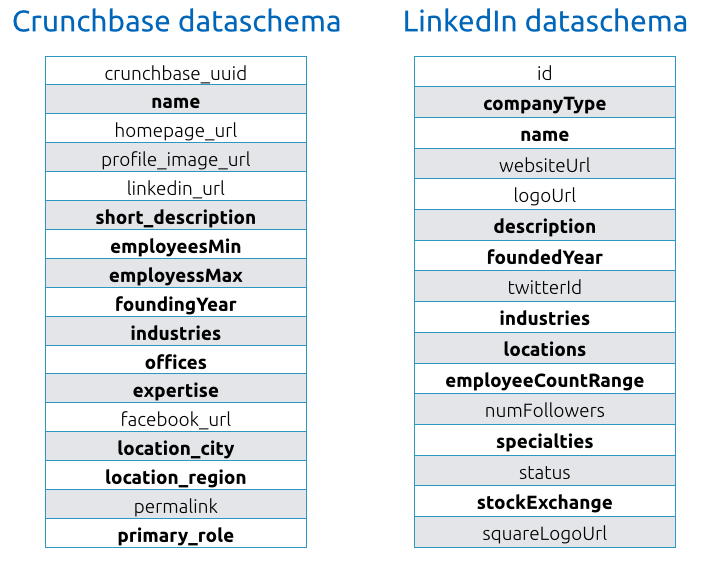
\includegraphics[scale=0.5]{sources_dataschema.png}
\centering
\caption{Comparison of dataschemas}
\label{fig:sourcesSchemas}
\end{figure}

\subsubsection{Datasources}
To ensure a good quality the data-sets were extracted from two different sources, LinkedIn and Crunchbase.

LinkedIn is a social business network with over 300 million user,\footnote{https://www.linkedin.com/about-us, 28th of June 2015} with people from all over the world. Apart
from user-profiles it also contains company-profiles with properties like year of foundation, industry or
number of employees. The information are maintained by the companies itself.

Crunchbase is an open database containing startup-activity and company information.\footnote{https://info.crunchbase.com/about/ 28th of June 2015} Company-datasets contain information
like employees, competitors, industry and basic information as well. Like the wikipedia information can be maintained by everyone,
which could lead to frequently updated information on the one hand, and to wrong information on the other hand.

Figure \ref{fig:sourcesSchemas} shows a subset of attributes of companies that are provided by each source. \footnote{More detailed information can be found on http://data.crunchbase.com/v3/docs/organization and https://developer.linkedin.com/docs/fields/company-profile }
The characteristics that represent information to conclude a companies demand are printed bold. \footnote{Regarding to influencing factors
and a companies environment in chapter 2 and 3. See also Chapter 4.3} Both datasets provide similar information but with a different structure.
For example the number of employees. Crunchbase provides 2 attributes one for the mininum value and one for the maximum value as integers
whereas LinkedIn delivers a string like ``1001-5000'' which requires further processing to extract the same information.

\begin{figure}[ht]
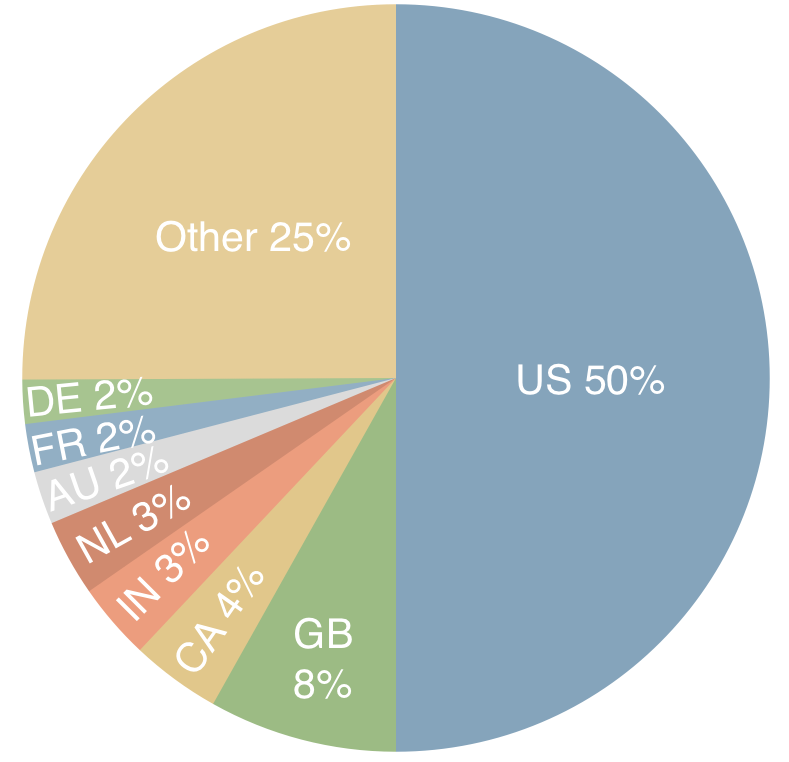
\includegraphics[scale=0.3]{companyCountries.png}
\centering
\caption{Distribution of companies per country (Total 236,235 companies)}
\label{fig:countryDistribution}
\end{figure}


\subsection{Dataprocessing}
Because both sources have different advantages and information and as mentioned in the last section a different structure,
it makes sense to combine both datasets into one, that covers all the necessary information needed for clustering,
and has one defined dataschema.

The biggest problem in combining these two datasets is finding the right corresponding company in the respectively
other dataset.
The used approach was to join to datasets on a 100\% match of both companynames. If companies have slightly different names
in both sets, they will be matched if they have the same website url given. Otherwise a new entry will be created in
the resulting dataset. This resulted in a dataset of 236,235 companies. As you can see in Figure \ref{fig:countryDistribution}
the most companies are located in the United States. The dataset contains companies from 220 countries.

[ Maybe add industries as well. ]




% Challenge: Finding a combination of Features which matches the closeness of companies
% to the need's development
\subsection{Company Features}
\label{companyFeatures}
Features are variables or a combination of variables that can describe certain characteristics of an entity. Using the right
features is essential to prove that strongly related businesses develop similar product needs. In this case the features have
to describe characteristics that influence a companies buying behaviour.

Regarding to Porter \cite{CompanyClusters} a company's \emph{location} has a high influence on how it acts. Companies will often rather know what happens next to
them than at a totally different place. Steps taken by companies right next to each other will have a higher impact on
how each of them reacts to particular circumstances, especially purchases made by one of the companies may lead to an economic
advantage. Other companies are then forced to close this gap by doing similar purchases.

Of course the location is important but has less impact if the companies next to each other do not compete somehow.
Referring to Porter \cite{CompanyClusters} companies of the same \emph{industry} are often shaped in clusters at one location.
They are using the same infrastructure and increasing the clusters know how.

So the first two features that cause the highest influence from one company to another are a company's location and its industry.

An increasing number of employees within a company leads to a higher complexity. Also bigger companies have other needs and higher expenses than
smaller ones have. Therefore companies of similar size are more related to each other than to smaller sized companies.
This leads us to the third feature, a company's size measured by its \emph{number of employees}.

According to Webster and Wind \cite{BusinessBuyingBehavior} companies are exposed to 6 different influences. These influences are already covered
by the selected features. For example by selecting a company's location the legal, economic and political influences which
are the strongest ones are considered.

Other characteristics mentioned in chapter 4.1 could also be used as features. But as the selected 3 features cover all the aspects
discussed during the economic background, there is no need for more features at the moment. A comparison of results using different combinations of
features could be part of future work. This thesis focuses on finding a correlation between the closeness of companies and their
demand-evolvement.

\subsection{Used Clustering Algorithm}

Some clustering approaches need to know the number of clusters. Of course one could estimate a number of clusters
by considering the number of industries as well as the number of different locations for each industry, but this would
still be an approximation to the number, which by the way would get invalid by adding more companies.
Hierarchical algorithms have the advantage that they do not need to know the number of used clusters. But this neither
solves the problem of getting good cluster because one would still have to figure out which of the multiple generated
clustering shemas should be used. So it is necessary to have a measurement of a cluster schema to find out which one
works best.

Furthermore the used clustering algorithms has to be exclusive and intrinsic. It would not be on purpose to find
characteristics on predefined groups but rather to define groups of companies. An exclusive approach would provide
the information to which cluster a company belongs.

% We will use a hierarchical clustering to group strongly connected companies.
%
% So our approach has to be, to get an evaluation of all companies according to their closeness to each other. This
% would also create some kind of clusters, but we would still have the information of closeness between each company.
% An appropriate datastructure to store this information is a graph.

The aim to explore and furthermore predict the need evolvement could be achieved by grouping strongly connected companies.
Companies that belong to one cluster should ideally have the same demands. To match the main thesis its important to find
correlations between closeness of companies and their needs. Especially its important that a cluster evolves exactly one same
need. This requirement makes to possible to allow predictions on a cluster's demand evolvement.

Therefore the approach will be to calculate the proximity between each of the companies. This makes it possible to
look for existing correlations and form clusters. A agglomerative hierarchical algorithm will be used to perform this.

As the algorithm produces different possible clusters a way to determine the best clusters is necessary. One clustercombination
has to fullfill the following characteristics:
\begin{itemize}
  \item All the clusters have a strong increase of exactly one demand each
  \item A cluster contains only companies that do not have the maximum possible proximity
\end{itemize}


\subsection{Calculate Proximity}
The calculation is performed on a randomly sampled subset of our total set of companies to save time and keep the amount
of produced realations as small as possible. The subset contains 1192 documents. This would result in a maximum count of
realtionships of 709.836, where each company has a relationship to each other, but not itself. Thats the result of following
function where n equals the number of companies.

\begin{center}
  { \Large #relations \LARGE = $\frac{n*(n-1)}{2}$}
\end{center}

For the proximity we take all of the features and weight them according to their influence. Regarding to the conclusions in chapter
\ref{companyFeatures} we assume that location and industry have a high weight whereas the company size does not have that much impact
on a company's buying behaviour.


\subsection{Cluster scoring}

To be able to evaluate which feature wheight is the best and which cluster combination of the set that emerges from the hierarchical
clustering it is necessary to have some characteristics to compare.

The first and most important one is the function score(X) that calculates how good a cluster is according to the fact whether
it strongly develops only one demand.

\begin{figure}[ht]
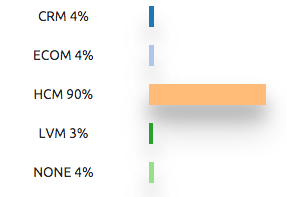
\includegraphics[scale=0.6]{goodCluster.png}
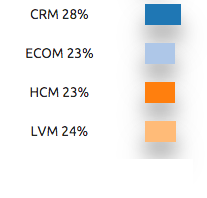
\includegraphics[scale=0.6]{badCluster.png}
\centering
\caption{A good and a bad example of a cluster's demand development}
\label{fig:clusterDemandDevelopment}
\end{figure}

Figure \ref{fig:clusterDemandDevelopment} shows a good demand development on the left and a bad one on the rigth. The used Dataset
of demand-posts covers 5 different products: CRM, ECOM, HCM and LVM. The percentage value says how many of the companies within
the according cluster raised a demand of the corresponding product.
The left distribution allows to conclude that the remaining companies in the cluster may also be interested in a HCM product.

\begin{figure}[ht]
  {
    \Large Let $X \subseteq \mathbb{Q}$ \newline
    \Large score(X) \LARGE = $\frac{ maxVal( ( max2(X) - avg2(X) ), 1 ) }{ ( max(X) - avg(X) ) }$ \newline \newline
    \large max(X) =  maximum value of set X \newline
    \large avg(X) =  average value of set X \newline
    \large max2(X) = $ max( X \textbackslash \{ y | y = max(X)\} )$ \newline
    \large avg2(X) = $ avg( X \textbackslash \{ y | y = max(X)\} ) $ \newline
  }
  \centering
  \caption{The scoring function}
  \label{fig:scoringFunction}
\end{figure}

The function score(X) returns a value that describes the ratio between the difference of the highest value and the
average to the difference of the second highest value and the average without the highest value. The closer the value
is to 0 the better the cluster.

If the highest value strongly differs from all the others than it has a high difference to the average value.
If the highest value is by far the highest than the difference between the second highest value and the average without
the higest value will small. To prevent a wrong result the denominator has to be at least 1 because otherwise the
whole value could be 0 even if the highest value does not have a high difference to the average.

To clarify the formula we are going to calculate for the two examples in figure \ref{fig:clusterDemandDevelopment}
The Left distribution:
\begin{center}
  score([4,4,90,3,4]) =  {\Large $\frac{ maxVal( ( 4 - 3,75 ), 1 ) }{ ( 90 - 21 ) } = \frac{ 1 }{ 69 } =$} 0.0144 \\
\end{center}

The right distribution:
\begin{center}
  score([28,23,23,24,6]) =  {\Large $\frac{ maxVal( ( 24 - 19 ), 1 ) }{ ( 28 - 20,8 ) } = \frac{ 5 }{ 7,2 } =$} 0.6944 \\
\end{center}


The left distribution has as expected a better value than the right distribution. To evaluate a whole cluster combination
the rating for each cluster gets calculated. All the ratings will then be averaged according to the clusters size.
So a good rating within a small cluster will not have as much impact as a good rating in a bigger sized cluster.

Other measurments to value a cluster combination are the total number of companies within the clusters or the
highest average of a products demand. The more companies covered, the more efficient the demand predictions are.
Also the higher the average covering is for the products, the more actively are the companies spreading demands
within a cluster. An average covering takes only the highest coverage from each of the existing clusters and averages
them. According to our exmaple in figure \ref{fig:clusterDemandDevelopment} we would calculate the average of 90 and 28.

























% {\small
% \begin{tabular}{ccccccc}
%   Clusters & Avg Rating & Level & High Avg & Big Cluster & Weight Sz In Lo & Tree depth \\
%     5 & 0.7969 & 28 & 38\% & 1049 & 0,0,1 & 777 \\
%     6 & 0.9860 & 67 & 22\% & 217 \(561\) &  1,0,0 & 284 \\
%     6 & 0.9860 & 67 & 22\% & 217 \(561\) &  0,0,1 & 284 \\
%     6 & 0.7001 & 47 & 48\% & 12 \(34\) & 1,1,1 & 59 \\
%     8 & 0.7375 & 51 & 45\% & 10 \(42\) & 2,4,1 & 61 \\
%     8 & 0.8693 & 41 & 47\% & 9 \(39\) & 2,2,1 & 50 \\
%     5 & 0.7125 & 10 & 39\% & 1086 \(1097\) & 2,8,1 & 63 \\
% \end{tabular}
% }

	\clearpage

	\section{Evaluation}

This section evaluates the result of different clusterings with different weights of the used features.
Multiple clusterings with different feature weight were processed to get a deeper understanding
of the correlation between the features and the demand development.

{\small
\begin{table}[ht]
  \caption{Different feature weights and their result}
  \label{table:clusteringComparison}
  \begin{tabular}{cccccccc}
    Nr. &  Clusters & \head{1.5cm}{Avg Rating} & \head{1cm}{Level} & \head{1cm}{Highest Avg} & \head{1cm}{Big Cluster} & \head{5cm}{Weight\newline{\small Size | Industry | Location}} & \head{1cm}{Tree depth} \\ \hline
    1&          8      & 1.0500     & 45    & 34\%     & 732 \(911\) &  0,0,1          & 777 \\
    2&          4      & 1.0560     & 119   & 22\%     & 233 \(357\) &  0,1,0          & 352 \\
    3&          3      & 1.0356     & 148   & 27\%     & 136 \(211\) &  1,0,0          & 284 \\
    4&          4      & 0.7597     & 61    & 27\%     & 46 \(64\)   &  1,1,1          & 107 \\
              %8      & 0.7375     & 51    & 45\%     & 10 \(42\)   & 2,4,1           & 61 \\
    5&          7      & 0.8480     & 51    & 7\%      & 43 \(94\)   & 2,2,1           & 94 \\
    6&          6      & 0.8556     & 60    & 7\%      & 43 \(99\)   & 2,8,1           & 103 \\
  \end{tabular}
\end{table}

}

\subsection{Correlation of company closeness and need development}

Table \ref{table:clusteringComparison} shows the resulting measurements regarding to the different feature weights.
To see what impact each feature has without the influence of the other ones, an own cluster combination for each
feature was created \footnote{See tablerows 1-3 in \ref{table:bestClustering}}.

The results for this combination were quite similar. Their average rating is between 1.03 and 1.05 whereas
the tree depth differs a lot. A hierarchical clustering always produces a tree as its outcome structure. This
tree represents the clustering. Each node within this tree represents an own cluster that contains every child element
of this node. So the deeper the tree the more one company clusters \footnote{A one company cluster is a cluster with only one element}
it contains. One company clusters are bad for deducing a correlation of company closeness and need development because
a company within a one company cluster can not have influence on any other companies within this cluster.
According to the results for clusterings with single weights only, the clustering resulted from the location weighted
tree has a much higher depth than any other result set. Therefore the location itself as a result is useless.
The other two single weighted trees are useless for predictions as well. Their clusters show a balanced demand
development for each of the products. So they are not suited for demand predictions by themselves.

This result is not astonishing as economic processes are very complex and can not be described by a single
measurement. Thats why we had a look at the influence of all three of the features. According to
Porter \cite{CompanyClusters} and Webster and Wind \cite{BusinessBuyingBehavior} industry and location
do both have a high influence. So we had a look at combination where this features where wheighted more than
the size feature.

The unexpected result was that the evenly ditributed weight to all of the three features leads the best outcome.
It has a similar depth like table rows number 5 and 6 but much better average rating which is the most interesting
measurement to look for. Even if it only covers two thirds of the other two result sets it has a higher prediction potential.

\begin{figure}[ht]

\includegraphics[scale=1]{bestClustering.png}
\centering
\caption{Visualized cluster for the cluster combination with the best rating}
\label{fig:bestClustering}
\end{figure}

Figure \ref{fig:bestClustering} shows the 4 clusters belonging to table row number 4 and the distance between each
of the cluster. One company clusters are ignored in this visualization because they do not provide any
further value. Even if this cluster combination provides the best average rating it is still not good enough
to perform any useful predictions. On the one hand it covers only around a twentieth of the overall companies set
and on the other hand the cluster score of 0.75 is still to high for reliable demand forecasts.

% why or why not may companies raise certain needs ~
\subsection{Improving the result}
\label{section:improvingResult}
The result proves an existing correlation between the used features and the demand development. But still
the outcome is not sufficient enough. Obviously the used characteristics do not cover up the whole complex
structure that describes the buying behaviour of companies.

One approach to solve this problem is to use more characteristics. Appropriate ones could be the monthly income,
a more detailed company descriptio or other metrics for a company's economic situation.

	\clearpage

	\section{Conclusion}
This thesis presented an approach to group companies, evaluate different clusters regarding
to their need development and predict demands of companies.

This thesis could not give the final answer to the problem, it is further more a
proof of concept that the primary objective to identify and current and future product
needs is possible.

The opportunities are promising. Knowing companie's demands beforehand would create a big
advantage to the ones using it.

\section{Future Work}
As this thesis is more a proof of concept than a final solution the main aspect of the
future work will be to improve the clustering by refering to more metrics as already mentionen
in section \ref{section:improvingResult}. Therefore it could be useful to also mention additional
datasources like the Compustat database which provides financial, statistical and market information
on companies throughout the world.

Another important part would be to enable the tool to work on huge datasets and implement the prediction
part to gain value from the obtained conclusions.

	\clearpage

	%%% BIBLIOGRAPHY
	%\bibliographystyle{babunsrt3-fl}
	\addcontentsline{toc}{section}{Bibliography}
	\bibliographystyle{babunsrt-fl}
	\bibliography{projektbib}

\end{document}
